\documentclass[10pt,a4paper]{article}
\usepackage[latin1]{inputenc}
\usepackage{a4wide, graphicx, clrscode, parskip}
\author{J.P.H. Snoeren (0772658) \and R. Stoof (0767157)}
\date{\today}
\title{2IDC0 Artificial Intelligence: International Draughts}
\begin{document}
\maketitle
\textbf{This report describes our artificial intelligence player for international draughts. To create this player, we have implemented the alpha-beta search algorithm. This algorithm uses a heuristic evaluation function to determine the value of a state in order to guide it to victory.} 

\section{Algorithm}
\subsection{Alpha-Beta Pruning}
Our computer player attempts to determine the best move that he can do in the current state. In order to find this best move, it evaluates all possible moves for a given game-state, with the assumption that his opponent will always make the best move on his behalf. In a zero-sum game, this means that our player attempts to maximize the value of the heuristic evaluation function, whereas the opponent tries to minimize it. The computer player finds his best possible move by using the alpha-beta algorithm, as explained during the lectures of the course. The alpha-beta algorithm is an extension of the minimax algorithm, in which pruning removes unnecessary calculations. The concept of the minimax algorithm is very simple. First, the value of the leaves is determined with the help of the heuristic evaluation function. Then, the value in the parent node of the leaves is chosen by either choosing the move that minimizes or maximizes the heuristic, depending on whether the node is for the maximizer or the minimizer. This recursively goes on until a best move for the root of the game-tree has been found.

Alpha-beta pruning attempts to prune sub-trees in the search tree, by checking whether it is necessary to search in a sub-tree. If we are sure that the value of the parent of the root in a certain sub-tree will not be greater (or higher) than the value to compare with, we can prune the sub-tree. \textsc{AlphaBetaPruning} presents pseudo-code for the implemented algorithm. The algorithm takes as input a node \emph{node}, two values $\alpha$ and $\beta$, the current depth and a boolean \emph{max} indicating whether the player that is calling the algorithm is the maximizing player or not.

\begin{codebox}
\Procname{$\proc{Alpha-Beta}(node, \alpha, \beta, depth, max)$}
\li \If \id{node} is a leaf node
\li	\Then
		\Return value of the evaluation function
	\End
\li \For all possible moves
\li	\Do
 		\If stopped
\li 	\Then
 			terminate the algorithm
 		\End
\li Do the next move
\li \id{newNode} = node corresponding to the current state
\li \id{childValue} = \proc{Alpha-Beta(\id{newNode}, $\alpha$, $\beta$, \id{depth} - 1, $\neg$ \id{max})}
\li Undo the move
\li \If \id{max}
\li \Then
	 $\alpha = \textbf{max}(\alpha, \id{childValue})$
\li \Else
	$\beta = \textbf{min}(\beta,\id{childValue})$
	\End
\li \If $\alpha \geq \beta$
\li 	\Then \If \id{max}
\li			\Then \Return $\beta$
\li		\Else
			\Return $\alpha$
		\End
	\End
\End
\end{codebox}

The algorithm \textsc{Alpha-Beta} finds the best move to be done in a search tree. Line 1 and 2 form the base case: When the node is a leaf node we simply return the value of the evaluation function. If the node is not a leaf, we check all moves that are possible from this node. Line 4 and 5 take care of stopping the algorithm. We simply terminate the algorithm (for instance by throwing an exception) once some external source told us to stop. We try to do a move in line 6 and recurse on the node corresponding to the state of the game after that move has been done. In line 9 we undo the move again. Line 10-12 update the values for $\alpha$ and $\beta$ accordingly, making the interval in which to search for the values of the evaluation function smaller. Line 13-16 performs the pruning of the algorithm. If $\alpha > \beta$, we can prune the search tree and return the value for $\alpha$ or $\beta$ immediately.

\subsection{Iterative Deepening}
Since the search tree will be very big, or maybe even infinite, it is not possible to search the complete tree. In the implementation there will be a time limit for the computer player to think about its move, so we would like to stop the search at a certain depth. However, it is rather hard to determine a depth at which to stop. If we stop too early, we waste time that we could have used to find an even better move. If we stop too late, we won't even have returned a move at all, and will be indecisive in what to do. To solve this problem, we use iterative deepening. We first run the algorithm on a tree of depth 1. Then we increase the depth and run the algorithm on a search tree of depth 2. Continuing in this fashion, we attempt to reach a depth as high as possible, but are able to stop when the time limit has run out. Algorithm \textsc{Iterative-Deepening} displays this approach using pseudo-code. It takes as input the current state of the game \emph{state}.

\begin{codebox}
\Procname{$\proc{Iterative-Deepening}(\id{state})$}
\li $\id{node} \gets$ New node representing \id{state} containing a \emph{best-move}.
\li $\id{depth} \gets 0$
\li \While $\neg$ stopped
\li \Do 
		\proc{Alpha-Beta}(\id{node}, $-\infty$, $\infty$, \id{depth}, \const{true})
\li 	$\id{depth} \gets \id{depth} + 1$
	\End
\end{codebox}

\subsection{Abortion}
In order to stop, we need to stop executing our algorithm in the middle of the execution. We achieve this by simply throwing an exception when the time limit has run out. In our implementation, this is achieved by a self-written exception, namely an \textsc{AIStoppedException}. When this exception gets raised, the player will jump out of the recursively looping algorithm.

\section{Heuristic evaluation function}
\subsection{Global evaluation function}
The algorithm described above would be utterly useless without a sophisticated evaluation function. If the heuristic is good, we can find the best move quickly with the help of the alpha-beta algorithm, creating a very strong computer player. Our evaluation function consists of different components combined together, in order to give a certain game-state a score. In fact, these components are used in a weighted linear function to compute the value of the state the game will be in. This means that our evaluation function $H$ will be of the form $$H = \sum^n_{n = 1} w_n \cdot h_n$$ where $w_1 \dots w_n$ are the weights of the different components, or sub-heuristics $h_n$ in the evaluation function. Further in this section we discuss the various components of our evaluation function. From this point onward we assume that our computer player plays with the white pieces and the white pieces are placed at the bottom of the board. If the player is in fact the black player, the same reasoning applies, but the logical is trivially 'mirrored'.

\subsection{Material}
By far the most important component of the evaluation function is the material present on the board. For each white piece the value of this component goes up, but for each black piece this same value is subtracted. This means initially that the value of this component will be 0, as both players have an equal amount of pieces, which are all of the same type (non-king). If the computer player can sacrifice one of its pieces such that it can kill off more than one pieces of the human player, it will often do so. It is possible however that the other heuristics combined decrease the heuristic value in the end however, which means it's not worth to sacrifice the piece.

Because of the fact that \emph{kings} can go backwards and move multiple squares in a single move. they are more valuable. In our implementation, kings are three times more valuable than normal pieces. This ratio was found by no other means than our intuition.

\subsection{Crownpiece}
The crownpiece is the piece residing at location 48 (or location 3 in case of the black player), as can be seen in figure \ref{crownPiece}. Note that the black squares are numbered from left to right and from top to bottom, as you would read a book. On top of that, the numbering starts with the number 1. This piece, or actually the location on the board, is important. A piece on this location can go either to the left or to the right on the board, and can help on the side where help is needed.

Other pieces are in general restricted, since they are already placed on the left or right, or they are too close to the opponent's pieces. However, the crownpiece should not have a weight that is too high, since at some point the player should let go of the good position of the crownpiece in order for it to be useful. In our implementation, we have chosen the value of the piece to be 20\% as big as a normal piece.

\begin{figure}[h!]
	\begin{center}
	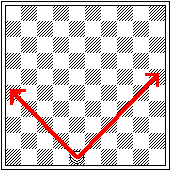
\includegraphics{./images/crownPiece.png}
	\caption{The crownpiece can reinforce both sides of the board. $^{[1]}$}
	\label{crownPiece}
	\end{center}
\end{figure}

\subsection{Zoning}
The board can be divided in three zones. The left zone consists of the three leftmost columns, the middle zone of the middle four columns and the right zone of the three rightmost columns, as displayed in figure \ref{zoning}. It might be a good strategy to divide the pieces according to the pieces of the opponent. In figure \ref{zoning} for example, we can see that we have three pieces in the right zone, but our opponent has five. It might be a good idea to balance the number of pieces in the zone, such that the opponent cannot easily breach through our defences and obtain a king.

\begin{figure}[h!]
	\begin{center}
	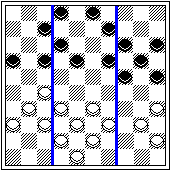
\includegraphics{./images/zoning.png}
	\caption{Dividing the board in zones to have a better defence. $^{[1]}$}
	\label{zoning}
	\end{center}
\end{figure}

\subsection{Clustering}
In international draughts, the structure of your pieces is important. Lone pieces can easily be captures or lured into tricks, but pieces next to each other or close to each other can help the player drastically. Thus, we include some notion of this "closeness" in our evaluation function. We do this in the form of clustering. Each space on the board has four neighbouring pieces, namely at its diagonals. This component of the evaluation function gives a higher value whenever the a piece has more neighbours. This (hopefully) makes sure that pieces will not go on lonely quests for victory, but take a more structured approach and stick together. In fact, because every piece will try to form these X-formations, it is highly likely that big defensive lines will be formed. Do note however that for these formation we only consider normal pieces. Because of freedom of movement kings have, we do not think kings should participate in the clustering.

With that into consideration, our implementation is such that each piece gets an additional 20\% of its original value for each diagonal neighbour. That means, if a piece is in the middle of an X-formation, it can gain an additional maximum score of 80\% of its original value, since it can have at most 4 diagonal neighbours.

\subsection{Depth on the board}
Another factor we might use in the evaluation function is how far the pieces are on the board. Pieces being closer to the front are more valuable than others. Pieces at the bottom of the board are not useful at all for attacking and their defence is usually very limited. In general it is a good strategy to move these pieces away from the bottom of the board to make them more useful.

Furthermore, being closer to the opponent's side of the board creates extra opportunity for obtaining a king. So we enhance our evaluation function with a component which favours pieces at the top rows (for white pieces). The additional score is linear to the amount of rows it has progressed. That is, if a piece has advanced $n$ rows, it will have an additional score of $n$. Just like with the clustering heuristic however, this heuristic is not implemented for kings, as it does not make sense for a king to stay on one side of the board.

\subsection{Analysis of the function}
During the development of the evaluation function, we tested each new heuristic against other players, which could be either human players, random players or previous  versions of our computer player. Based on these tests, we select appropriate weights for the evaluation function and determine whether certain aspects need to be included or not. Thus, the final heuristics function was created with a bottom-up approach, where sub-heuristics were added to our global heuristic function and tested against previous iterations that did not include the added sub-heuristics.

Our most important finding was that the zoning component did not make much sense in the evaluation function. After testing our computer player with zoning against the computer player without zoning multiple times (about ten times), we found that the computer player \emph{without} zoning won all of the games. This observation made us decide to drop the zoning component from our evaluation function altogether. Every other extension of the global heuristic led to a better player that won from all previous global heuristics.

\section{Contributions}
Both of us (Roy Stoof and Jacco Snoeren) worked on the project simultaneously, one typing the code and the other thinking along. Other aspects of the project, including planning what to do next and which aspects to include in the evaluation function were done together as well. Sometimes (manual) testing was done during the coding, to find out where the computer player made errors and how improvements could be made. This report is written by both of us as well.

\section{Manual}
In this section, we give a short manual on how to reproduce the results of the project. 

\begin{enumerate}
\item Run the project AICompetition. The interface for the game appears.
\item Press "Create schedule". A popup appears.
\item Select the players that you want to include and press "OK".
\item The panel on the right shows all possible matches that can be played. A distinction is made between the match where player 1 is white and player 2 black and vice versa. Choose a match that includes our computer player, which is named "Group-43".
\item Try to beat our player with your own skills (either international draughts skills or programming skills). 
\end{enumerate}

\section{References}
$^{[1]}$ http://dezlaren.home.xs4all.nl/opgaven/techniek.htm (Images \& Tactics)
\end{document}